\section{Three-Dimensional A–φ Fields and Diagnostics}
\label{chapter:08}

% block-id: 08.aphi.p1
\hypertarget{08.aphi.p1}{}
The A–φ model recovers current using \eqref{eq:E07} from saved A and actual gradients of φ. The three cylinder meshes contain 1683, 3672, and 9108 nodes; results appear in Fig.~\ref{fig:aphi_gates}. Radial J calibration meets its target on the finest mesh, while φ and gauge residuals fail on all three; the two coarser meshes also fail the J target. Manufactured-solution checks support correspondence between the tested equations and implementation, while physical cylinder calibration reveals field–potential consistency questions requiring further research.

% block-id: 08.aphi.p2
\hypertarget{08.aphi.p2}{}
Fig.~\ref{fig:aphi_preserved} uses 128 explicitly identified nodal samples to display A, φ, J and the actual φ gradient at those locations. The reproduction materials retain boundary, scaling, derivative and postprocessing diagnostics, together with failure causes for direct factorization, out-of-core and iterative routes. These records help distinguish implementation problems from discretization errors. The current cylinder results have not passed physical acceptance.

% block-id: 08.equation.E07
\hypertarget{08.equation.E07}{}
\hypertarget{E07}{}\begin{equation}\mathbf J=-\sigma\left(j\omega\mathbf A+\nabla\phi\right)\tag{8}\label{eq:E07}\end{equation}

% block-id: 08.figure.aphi_preserved
\hypertarget{08.figure.aphi_preserved}{}
\begin{figure}[!htbp]
\centering
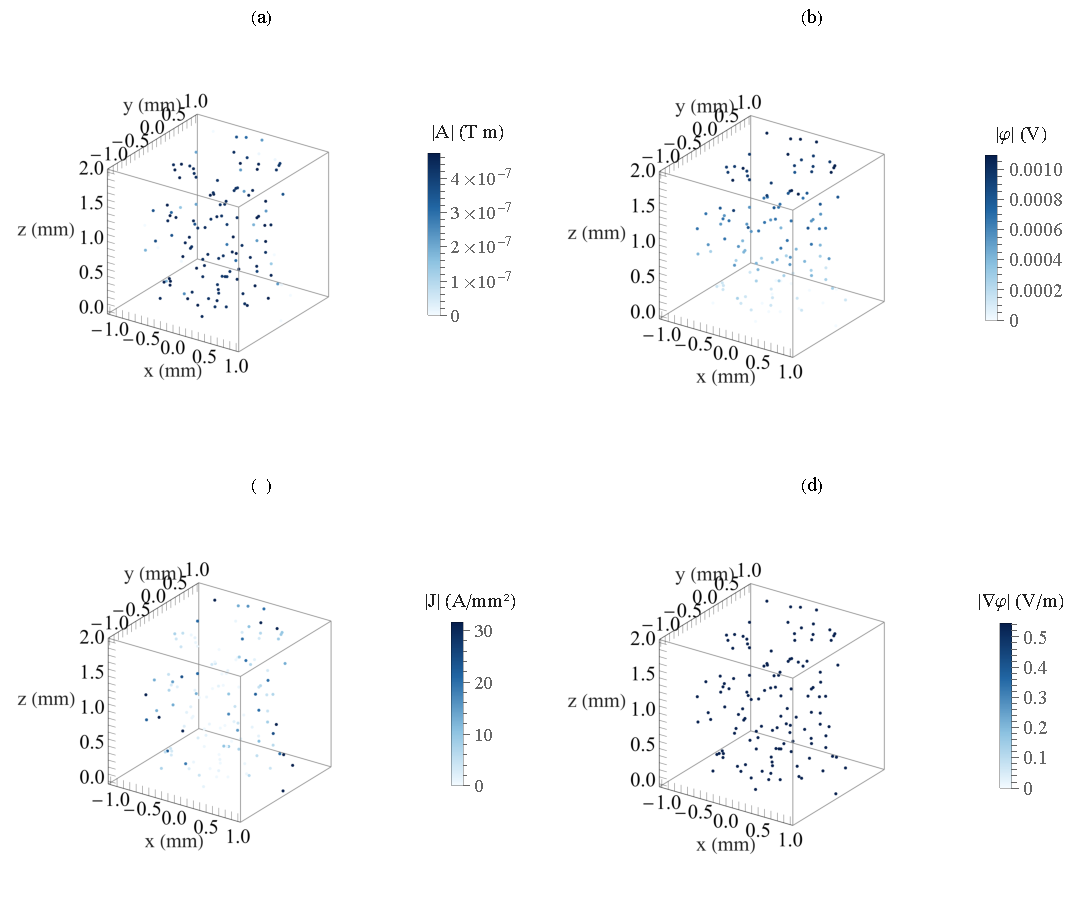
\includegraphics[width=\linewidth,height=.72\textheight,keepaspectratio]{../../assets/en/aphi_preserved.pdf}
\caption{Preserved A–φ field samples. Panels show A, φ, J, and the actual gradient of φ. The 128 selected nodes retain their sample identities. Color scales use magnitudes of the actual saved complex fields and derivatives.}
\label{fig:aphi_preserved}
\end{figure}

% block-id: 08.figure.aphi_gates
\hypertarget{08.figure.aphi_gates}{}
\begin{figure}[!htbp]
\centering
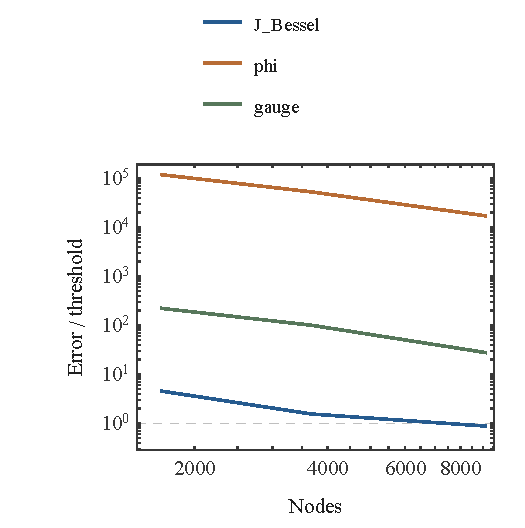
\includegraphics[width=\linewidth,height=.72\textheight,keepaspectratio]{../../assets/en/aphi_gates.pdf}
\caption{A–φ cylinder calibration metrics. Three grids and their metric targets are shown separately. The three cylinder levels contain 1683, 3672, and 9108 nodes. Errors are normalized by their respective acceptance targets, with the horizontal line indicating a unit ratio.}
\label{fig:aphi_gates}
\end{figure}
